\FloatBarrier
\section{N-body Problems}
If we consider an N particle/body problem formed of $N$ potential/quadrature points $\{{\bm{x}}_n\}$ each with an associated potential/force $\{{\bm{f}}_n\}$ that we will evaluate at the same set of points then we can compute the velocity at each $\bm{x}_n$ where $n=1,2,\dots,N$ through
\begin{equation*}
    \bm{u}(\bm{x}_n) = \sum_{i=1}^N \Phi(\bm{x}_n,{\bm{x}}_i){\bm{f}}_i
\end{equation*}
where $\Phi$ is the green's function associated with the underlying partial differential equation governing the dynamics of the system.

Systems of this form occur in a variety of problems such as electrostatics, heat conduction and stokes flow \cite{Cortez2015, Beatson, Tornberg2008, Greengard1990APotentials}. If the matrix-vector  product is computed directly then the calculation of the velocities for a $N$ body needs $\mathcal{O}(N^2)$ operations which, for a large number of particles, quickly becomes prohibitive due to rapid growth in the number of operations. For large scale systems where we need to consider hundreds, thousands or even millions of particles this becomes impossible even with modern hardware. To compute systems on this scale, we need to apply a different algorithm that can approximate this solution with fewer operations. 

\subsection{Barnes and Hut Algorithm}
The first method proposed to compute these systems was proposed by Barnes and Hut \cite{Barnes1986} and is a tree-based approximation of N-body simulations. By using a Quadtree in 2 dimensions or Octree in 3 dimensions [decomposition of the domain][not needed?] we can reduce the number of computations needed in the problem to $\mathcal{O}(N\log N)$. Tree-based decomposition uses a tree data structure to bin particles in smaller domains in which we can consider particle to particle interactions for particles close to each other and an approximation of the particle for particles further away. Barnes and Hut's algorithm uses the algorithm described in \cref{alg:BarnesHut} to reduce the number of calculations. 

\subsubsection{Decomposition of domain}\label{sec:Decomposition}
The basis of the Barnes and Hut algorithm is the decomposition of the domain into a tree-like structure [think you've covered this in the paragraph above?]. At level 0 we take the entire computational domain of the problem which includes all points. Level 1 divides the computation domain into even sections, 4 nodes in two dimensions or 8 nodes in three dimensions. At each level $2,\dots,l$ we subdivide the previous levels nodes creating nodes that are the children of the box [what is a box, not mentioned previously?] above them called the parent. This is done repetitively until the number of points in a box is at most 1 as shown in \cref{fig:2DDecompostion}.

\begin{figure}
    \centering
    \includegraphics[width=0.5\textwidth]{Images/KIFMM/Decomposition.pdf}
    \caption{An example of two-dimensional decomposition of a domain for use in the Barnes Hut algorithm and original FMM algorithm.}
    \label{fig:2DDecompostion}
\end{figure}

\subsubsection{\texorpdfstring{The $\mathcal{O}(N\log N)$ algorithm}{The O(NlogN) algorithm}}

In order to reduce the number of calculations needed we need to group particles together where appropriate. Physical intuition gives us a standing [??] that if a cluster of particles lie close enough together and far enough away [from what], we can safely and accurately replace the sum over each individual particle with a single term based on those particles' total mass and centre of mass. We will refer to this cluster size to distance ratio as $\theta$. We have already defined a kind of clustering based on the decomposition of the domain described above [where?]. If we start from the lowest nodes and work our way up the tree in post-order (see \cref{appendix:Tree}) we can calculate the centre of mass and total mass for all the particles below it. For nodes at the top of the tree on level $l$, this is simply the node's position and mass. Nodes in level $l-1$ will consider the 4/8 particles in its children boxes, nodes in level $l-2$ will consider the 16/64 particles beneath it and so forth up to the root node at level $0$. This is computationally demanding towards the top of the tree where all $N$ particles need to be considered, however, we can calculate the centre of mass of a node as the weighted sum of the centres of masses of the children nodes. This dramatically reduced the number of computations needed to compute the centre of mass of each node of the tree. 

Now that all nodes have a total mass and centre of mass associated with them, we can compute the force on a single particle. Considering each particle in the tree we traverse the tree in pre-order (see \cref{appendix:Tree}), that is from the root node down, considering each children node in turn. If the width of a node divided by its distance from the considered particle is smaller than $\theta$, which typically takes a value of $1$, then we consider all the particles beneath it clustered enough and far enough away that we only need consider that nodes' total mass and centre of mass. We stop the traversal of that branch of the tree and move on to the next branch dictated by the pre-order traversal. If a node is close enough that we cannot consider it clustered, then we look at the children of that node and see if any children nodes can be considered clustered enough to use that nodes centre of mass. This is repeated recursively until we have reached the bottom of the tree where we consider particle to particle interactions.

\begin{algorithm}[ht]
\caption{The Barnes-Hut Method}\label{alg:BarnesHut}
\begin{algorithmic}
\State Define distance threshold $\theta$
\State Decompose the domain into a tree structure until there is one particle per node
\For{Each node in post-order (see \cref{appendix:Tree})}
\If{Node has 1 particle}
\State Centre of mass and total mass equals the position of particle and mass of the particle
\Else 
\State Calculate centre of mass and total mass from children nodes
\EndIf
\EndFor
\For{For each particle traverse the tree in pre-order (see \cref{appendix:Tree}) to compute total force on the particle}
\State Let $D$ be the size of the node $n$ and $r$ be the distance between the particle and the centre of mass of node $n$
\If{$n$ has one particle}
\State compute the force between particles 
\Else
\If{$D/r < \theta$}
\State Compute the force on the particle from the centre of mass and total mass of 
\State $n$
\Else
\State Calculate the force based on the children of node $n$
\EndIf
\EndIf
\EndFor
\end{algorithmic}
\end{algorithm}

The Barnes-Hut method performs N-Body simulation very efficiently and is incredibly simple to implement. In most cases it achieves an error of about $1\%$, however it can perform much worse in highly clustered problems. Due to its easy implementation it is still used widely, particularly in astrophysical simulations \cite{Gaburov2010,Capuzzo-DolcettaIstitutoAstronomico,Ishiyama20124.45Problem,Iwasawa2019ImplementationC,Rein2013Large-scaleRings}.

\subsection{The original FMM algorithm}
While the Barnes-Hut method performs well for certain systems it is limited by the accuracy of the results that it can obtain. Based on the same domain decomposition as the Barnes-Hut method, the Fast Multipole Method (FMM) proposed by Greengard and Rokhlin \cite{1988The0-262-7110-X.,Rokhlin1985RapidTheory,Greengard1987ASimulations} provides a faster and more accurate method for computing N-body problems. Rather than purely computing with forces as in the Barnes-Hut algorithm, the FMM uses potentials to calculate the interaction between particles. By using potentials, the FMM algorithm can use more complex multipole expansions to calculate the interaction between distance [distant?] particles. By doing this expansion we can reduce the number of operations required to $\mathcal{O}(N)$ in optimal cases.

FMM algorithms look at problems in which the kernel $\Phi$ of the problem obeys the Laplace equation \cite{Beatson}. In order to both simplify the explanation and the mathematics involved in the original Fast Multipole Method \cite{Greengard1987ASimulations} , we will consider the problem of the Coulomb's potential in two dimensions. If we are given a two dimensional point charge of magnitude $q$ located at a point $\bm{x}_0 = (x_0,y_0) \in \mathbb{R}^2$ in polar coordinates, then we can calculate the potential at a point $\bm{x} = (x,y)$ as given by
\begin{equation*}
    \phi(x,y) = -q\log(\lVert \bm{x} - \bm{x}_0 \rVert)
\end{equation*}
which when away from source points obeys Laplace equation in two dimensions
\begin{equation*}
    \nabla^2 \phi = \frac{\partial^2 \phi}{\partial x^2} + \frac{\partial^2 \phi}{\partial y^2} = 0
\end{equation*}
In order to simplify notation, we will consider a relationship between the point $(x,y)$ and a complex point $z$. We can do this as the potential $\phi$ is a harmonic function as it obeys Laplace's equation, so there exists an analytic function $w$ for which $\phi = Re(w)$. In our case, this gives us that 
\begin{equation*}
    \phi(\bm{z}) = q\log(z-z_0)
\end{equation*}
In this form we can write the Taylor expansion of this potential given that $|\bm{x}|>|\bm{x_0}|$ as 
\begin{equation}
\label{eq:FMMOuterSingle}
    \phi(\bm{x}) = q\left( \log(z) - \sum_{k=1}^{\infty} \frac{1}{k}\left( \frac{z_0}{z} \right)^k \right)
\end{equation}
If we consider $n$ charges of strengths $\{q_i\}$ located at points $\{z_i\}$ where $i=1,\dots,n$ with $|z_i|<r\in\mathbb{R}$, then for any point $z\in\mathbb{C}$ with $|z|>r$, the potential $\phi(z)$ is given by
\begin{equation}
\label{eq:FMMOuterMulti}
\begin{gathered}
    \phi(z) = Q\log(z) + \sum_{k=1}^\infty \frac{a_k}{z^k} \text{ where }\\
    Q = \sum_{i=1}^n q_i \quad \text{ and } \quad a_k = \sum_{i=1}^{m} \frac{-q_i z_i^k}{k}
\end{gathered}
\end{equation}
which is simply the sum over \cref{eq:FMMOuterSingle} for all charges. We will refer to this as the multipole expansion. 

\subsubsection{\texorpdfstring{The exact $\mathcal{O}(N\log N)$ algorithm}{The exact O(NlogN) algorithm}}
If we consider the same hierarchical decomposition described in \cref{sec:Decomposition} where we have divided the domain into a set of nodes. For each set of nodes, we have 3 definitions that define a node's relation to other nodes in the tree.
\begin{itemize}
    \item Two nodes are said to be near neighbours if they are at the same level and share a point on their boundary. (A node is a near neighbour of itself.)
    \item Two nodes are said to be well separated if they are at the same level and are not near neighbours.
    \item With each node $i$ is an associated interaction list, consisting of the children of the near neighbours of $i$’s parent which are well separated from node $i$ [might need a graphic here to explain!]
\end{itemize}
We traverse down the tree from the root node, at level $0$ and one [?] $1$ we have no pairs of nodes which are well separated so we can skip over these two levels starting at level $2$. We can now use multipole expansions to compute the contribution to the potential of all particles in a node from other well-separated nodes. We still need to compute the interactions of particles in a node's current near neighbours which cannot be done by a multipole expansion. If we now look at the level below, some of the points in the nodes near neighbours are now in nodes that are well separated and as such their contributions can be computed by multipole expansions. This set of nodes is fully defined by the node's interaction list defined above. This process is continued until the bottom of the tree is reached and we compute particle to particle as we did in the Barnes Hut method. 

\begin{algorithm}[ht]
\caption{The exact NlogN Algorithm}\label{alg:FMMNlogN}
\begin{algorithmic}
\State Decompose the domain into a tree structure until there is one particle per node
\For{For each particle $i$ traverse the tree in pre-order (see \cref{appendix:Tree}) to compute total force on the particle}
    \State Decompose the domain 16/64 even nodes
    \State Compute the contribution of particles in nodes well separated from the node
    \State \; containing $i$ using multipole expansions.
    \Repeat
        \State Subdivide all nodes into 4/8 children nodes.
        \State For nodes in the interaction list of the node containing $i$ compute the 
        \State \; contribution of using multipole expansions
    \Until{One particle per node}
    \State Compute remaining interactions of near neighbour nodes directly
\EndFor
\end{algorithmic}
\end{algorithm}

This version of the Fast Multipole method computes in the same $\mathcal{O}(N\log N)$ as the Barnes Hut method, however it is capable of exact results due to the use of the multipole expansions. Numerically this is not possible as infinite terms are needed for each expansion, so we truncate the expansions to $p$ terms where each expansion has an error estimate of \cite{Beatson,Greengard1987ASimulations}
\begin{equation*}
    \left|\phi(z)-Q \log (z)-\sum_{k=1}^{p} \frac{a_{k}}{z^{k}}\right| \leq A\left(\frac{1}{2}\right)^{p} \text{ where } A = \sum_{i=1}^{n} |q_i|
\end{equation*}
where $n$ is the number of particles involved in the expansion. This means that at each level $\mathcal{O}(N)$ amount of work need to be done as we need to compute the multipole expansion for each particle at each level giving $\mathcal{O}(Np)$ operations. If we assume homogeneity, where the particles are evenly distributed then there will be roughly $\mathcal{O}(\log N)$ levels giving the overall complexity as $\mathcal{O}(N\log N)$ with the total cost being $27Np\log N + 8N$ where the $8N$ is the number of direct interactions and the factor of $27$ comes from the maximum size of the interaction list. 

\subsubsection{\texorpdfstring{The $\mathcal{O}(N)$ algorithm}{The O(N) algorithm}}
In order to reduce the algorithm from $\mathcal{O}(N\log N)$ to $\mathcal{O}(N)$ we need to make better use of our multipole expansion. We will derive translations of \cref{eq:FMMOuterMulti} both in $z$ and $z_0$ such that we only need to form the multipole expansion once per node.
By translating equation \cref{eq:FMMOuterSingle} and again summing over all charges we obtain that
\begin{equation}
\label{eq:FMMOuterMultiTrans1}
    \phi(z) = a_0\log(z-z_0) + \sum_{k=1}^\infty \frac{b_k}{(z-z_0)^k}
\end{equation}
We can again take the Taylor expansion of this with respect to $z_0$ to obtain the multipole expansion of a set of potentials located in a circle of radius $R$ centred at $z_0$ for a point outside a circle of radius $R+|z_0|$ with radius at the origin as 
\begin{equation}
\label{eq:FMMOuterMultiTrans2}
\begin{gathered}
    \phi(z) = a_0\log(z) + \sum_{k=1}^\infty \frac{b_k}{z^k} \text{ where } \\
    a_0 = \sum_{i=1}^n q_i \quad \text{ and } \quad b_k = -\frac{a_0 z_0^k}{k} + \sum_{l=1}^{k} a_l z_0^{k-l} \binom{k-1}{l-1}
\end{gathered}
\end{equation}
with $\binom{k}{l}$ being the binomial coefficients.

While \cref{eq:FMMOuterMulti,eq:FMMOuterMultiTrans1} allows us to calculate the potential away from a cluster of particles, we also need to consider the potentials inside a circle $D_1$. Considering a group of charges inside a circle $D_2$ with radius $R$ centred at $z_0$, with $|z_0|>(c+1)R$ with $c>1$. Then we can write the potential at the origin using \cref{eq:FMMOuterMultiTrans1}. We can then expand this potential locally about the origin to be able to calculate the potential at a point inside the circle $D_1$ of radius $R$ centred at the origin as
\begin{equation}
\label{eq:FMMInner}
\begin{gathered}
    \phi(z) = \sum_{k=0}^\infty \frac{b_k}{z^k} \text{ where } \\
    b_0 = a_0\log(-z_0) + \sum_{l=1}^\infty \frac{a_l}{z_0^l}(-1)^l \text{ and } \\
    b_k = -\frac{a_0}{k\cdot z_0^k} + \sum_{l=1}^{k} \frac{a_l}{z_0^{l}} \binom{l+k-1}{l-1}(-1)^l, \text{ for } l>0.
\end{gathered}
\end{equation}
This is obtained through a Maclaurin expansion about the point $z$, the full derivation can be seen in Beatson and Greengard \cite{Beatson}. 

\begin{figure}
    \centering
        \resizebox{.6\linewidth}{!}{\begin{tikzpicture}
    \node[anchor = south west,inner sep=0] (image) at (0,0) {\includegraphics[width=.6\textwidth]{Images/KIFMM/Translation.pdf}};
    \begin{scope}[x={(image.south east)},y={(image.north west)}]
    \begin{scope}[x={(image.south east)},y={(image.north west)}]
        \node at (0.32,0.2) {$R$};
        \node at (0.70,0.8) {$R$};
        
        \node at (0.27,0.26) {$0$};
        \node at (0.74,0.73) {$z_0$};
        
        \node at (0.57,0.46) {$(c+1)R$};
        
        \node at (0.78,0.6) {$D_2$};
        \node at (0.2,0.4) {$D_1$};
    \end{scope}
    \end{scope}
\end{tikzpicture}
}
    \caption{Source charges $q_1,\dots,q_n$ are contained in the circle $D_2$. The corresponding expansion about $z_0$ converges inside $D_1$.}
    \label{fig:Translation}
\end{figure}

We can also translate the centre of the Maclaurin expansion using the following.

\begin{equation}
    \label{eq:LocalTranslation}
    \sum_{k=0}^p a_k(z-z_0)^p = \sum_{k=0}^{p} \left( \sum_{l=k}^p a_k \binom{l}{k})(-z_0)^{l-1} \right)z^k
\end{equation}

These expansions have the benefit of allowing for the evaluations of multipole expansions without the need to sum over all particles within that node. In particular, if we have the multipole expansion for each of the children of a node we can use \cref{eq:FMMOuterMultiTrans2} to translate the centre of expansion for each node to the centre of the parent node and then add the expansion together. Equation \ref{eq:LocalTranslation} allows us to do the opposite, where, if we have an expansion that described the potential inside of node $b$ from all particles outside $b$'s near neighbours, we can use \cref{eq:LocalTranslation} to transmit this information to $b$'s children.

We will build on the $\mathcal{O}(N\log N)$ algorithm described in \cref{alg:FMMNlogN} and only note the differences in the two methods. Instead of decomposing the domain as we work our way down the tree we decompose the whole tree first as in the Barnes Hut algorithm. As we are forming multipole expansions we do not need to decompose the domain until we have a single particle in each node, instead we divide until there are at most $s$ particles per node at the finest level. As with the Barnes Hut algorithm, we work from the bottom of the tree in post order. For leaf nodes we form a truncated multipole expansion of $p$ terms based on the particles in the node. The expansions for all boxes in higher levels are then formed by shifting the expansions of all children nodes to the centre of the node and summing over coefficient terms.

Once we have expansions for each node we can traverse down the tree.
In the $\mathcal{O}(N\log N)$ algorithm we traverse down the tree for each particle $i$ using multipole expansions to compute the contributions of nodes in the interaction list of the node containing $i$. Instead we use \cref{eq:FMMInner} to expand the multipole expansion of nodes in the interaction list into a local expansion which is valid inside the whole node. This expansion can then be shifted to the children of the node using  \ref{eq:LocalTranslation} where we then consider the interaction list of the children nodes.  After traversing the whole tree we have formed a local expansion valid for each node at the finest level of the tree. We can evaluate these expansion at all particle positions and compute the direct interactions of particles in near neighbour nodes. This can be illustrated in \cref{fig:3Step} where we consider the interaction between two well separated nodes $A$ and $B$. If we assume that both nodes have $N$ particles in them, then computing the potential at all points in $B$ from all points in $A$ requires $\mathcal{O}(N)$ computations. The evaluation of the expansion at node $B$ is of order $\mathcal{O}(1)$ before the local expansion and evaluation requires another $\mathcal{O}(N)$ computations.

\begin{figure}
    \centering
        \resizebox{.6\linewidth}{!}{\begin{tikzpicture}
    \node[anchor = south west,inner sep=0] (image) at (0,0) {\includegraphics[width=.6\textwidth]{Images/KIFMM/3 Step.pdf}};
    \begin{scope}[x={(image.south east)},y={(image.north west)}]
    \begin{scope}[x={(image.south east)},y={(image.north west)}]
        \node at (0.25,0.9) {$A$};
        \node at (0.75,0.9) {$B$};
        
        \node at (0.25,0.22) {$C_A$};
        \node at (0.75,0.22) {$C_B$};
    
        \node at (0.5,0.78) {$\mathcal{O}(N^2)$};
        \node at (0.5,0.34) {$\mathcal{O}(1)$};
        \node at (0.35,0.5) {$\mathcal{O}(N)$};
        \node at (0.65,0.5) {$\mathcal{O}(N)$};
    \end{scope}
    \end{scope}
\end{tikzpicture}
}
    \caption{A diagram illustrating the 3 step process FMM's use to reduce the complexity of N-body interactions from $\mathcal{O}(N^2)$ to $\mathcal{O}(N)$}
    \label{fig:3Step}
\end{figure}

This 3 step approach for calculating the interaction between two boxes gives us a total order $N$ algorithm. In two dimensions the upwards pass takes $\mathcal{O}(Np)$ operation to calculate the multipole expansions for each node, $\mathcal{O}(29 \left(\frac{N}{s}\right) p^2)$ to shift the expansions between nodes, $\mathcal{O}(Np)$ operations to evaluate the local expansions and finally $\mathcal{O}(9Ns)$ operations to compute the near neighbour interactions. In 3d the total number of operations is of the order of $189\left(\frac{N}{s}\right)p^4 + 2Np^2 + 27Ns$. This means that the cost of increasing the accuracy of the original FMM algorithm in three dimensions grows by $\mathcal{O}(p^4)$, however, more recent work on the highly analytical structure of the FMM algorithm has allowed for the reduction of the cost of higher order multipole expansions. Through the rotation of the nodes the work needed to translate the expansions has been decreased to $\mathcal{O}(p^4)$ to $\mathcal{O}(p^3)$ \cite{Greengard1997ADimensions,Hrycak1998AnFields} and even to $\mathcal{O}(p^2)$ by diagonalising the translations \cite{Berman2006Grid-MultipoleCalculations,Elliott1996FastAlgorithm}, however these introduce numerical instabilities into the algorithm. The latest generation of FMMS are based on combining multipole expansions with plane wave expansions \cite{Greengard1997ADimensions,Hrycak1998AnFields} allow for numerically stable calculations in 3 dimensions with a dependence on $p$ of only $\mathcal{O}(p^2)$. 

The derivation of the multipole expansions and translations were done here in two dimensions and for the Coulomb potential [not sure this makes sense?]. Adaptation to 3 dimensional systems proves more analytically complicated but follows the same structure as the two dimensional case. Derivation of the multipole expansions typically involve the use of spherical harmonics, and the translations are more computationally complicated to evaluate. The adaptions to the algorithm can be seen in detail along with the full derivation of the expansions, translations and error estimates, in Greengard and Rokhlin (1987) \cite{Greengard1987ASimulations} and Beatson and Greengard (1997) \cite{Beatson}. The FMM is widely used and has been deployed in stellar dynamics as an improvement to the Barnes Hut algorithm \cite{Dehnen2014ADynamics}, in heat conduction \cite{Watschinger2021AEquation} and in non regularised stokes flow \cite{Selmi2007FastComplexity,Tornberg2008}. The only problem with the standard FMM's algorithms is the need to calculate multipole expansions for each kernel independently which can be difficult in cases such as in the case of the stokeslet kernel. We will look at an adaption to the FMM algorithm to create a kernel independent fast multipole algorithm (KIFMM) proposed by Ying \cite{Ying2004,Ying2005}.

\FloatBarrier
\section{Kernel-Independent Fast Multipole Method}\label{sec:KIFMM}
The KIFMM method retains the same structure as the original FMM algorithms but changes the way in which the potentials are represented and how the expansions and translations are computed. In order to remove the need to expand the kernel using multipole expansions we need an alternative method of accurately representing all particles in a node which requires less operations than the number of particles in the node. Ying \cite{Ying2004} proposes the use of equivalent surfaces which can capture the effect of the potential inside a node. We can then translate these surface potentials using only kernel evaluations and then evaluate the effect of these surfaces on the particle position.

In order to explain how the KIFMM method is adpated from the original FMM algorithm we will first explain how the KIFMM decomposes the domain. The main difference is the use of multiple interaction lists to evaluate the potential from different nodes. 

\subsection{Hierarchical decomposition of the computational domain}
We let $\mathcal{D}$ be the computational domain, which we define to be a cube in $\mathcal{R}^3$ such that it encompasses all points in $\{\bm{y}_n\}$ and $\{\bm{x}_m\}$. We typically define this to be the smallest possible cube which includes all the points. The KIFMM method in three dimensions builds an Octree structure of cubes in 3D with the cube $\mathcal{D}$ as the root node. We will label this node the Level $0$ partition where no subdivision has occurred. Each subsequent division is made of $8$ equal-sized cubes each with a side length of half of the cube above. For each level, we subdivide a node into its $8$ children when the number of source points or target points within the cube is greater than some threshold $s\geq 1$. For efficiency only points of the type which exceed the threshold are moved to the child nodes. This subdivision creates a new level $L+1$ containing the children of all subdivided nodes in level $L$. We refer to the node on level $L$ as the parent of nodes on level $L+1$. This process is repeated until all cubes have less than $s$ source or target points contained within them which we will refer to as leaf nodes.

\begin{figure}[ht]
    \centering
    \resizebox{.6\linewidth}{!}{\input{Images/KIFMM/3D OcTree}}
    \caption{A 3D example of a 4 level Octree generated on a set of random points (Points not shown). Black, red, blue and green cubes represents nodes on Level 1, 2, 3 and 4 of the Octree respectively.}
    \label{fig:Decompostionexample}
\end{figure}

An example of a simple decomposition can be seen in \cref{fig:Decompostionexample}. In the non-adaptive case, if any node has greater than $s$ source points, then all nodes on that level are subdivided creating $8^L$ new nodes. We might choose to implement a tree of this form when the potential distribution is uniform as it reduces the types and complexity of the interactions described later, but we will only consider the adaptive case in this discussion as it is more efficient in the non-uniform cases we will be considering.

\subsubsection{Interaction Lists}
For any node $B$ in the Octree, we define its relation to its neighbouring node[s?] through 4 interaction lists $I_U^B, I_V^B, I_X^B$ and $I_W^B$.

\begin{itemize}
\item The list $I^B_U$ contains $B$ itself and all leaf nodes which are adjacent to $B$. The $U$ list is empty for any non-leaf nodes.

\item The list $I_V^B$ contains all nodes which are children of the nodes which are neighbours of $B$'s parent. This means all nodes in $I_U^B$ are of the same level as B.

\item If $B$ is a leaf node then the interaction list $I_W^B$ contains all descendants of $B$'s neighbours whose parents are adjacent to $B$ but are not adjacent to $B$ themselves. In order to avoid computing the effect of the node twice we only include nodes $A$, where $A$ and all its decedents, obey the condition[s?] above. If $B$ is not a leaf node then $I_W^B$ is empty.

\item The list $I_X^B$ contain all nodes $A$ in which $B$ appears in the interaction list $I_W^A$.
\end{itemize}

\begin{figure}[ht]
    \centering
    \resizebox{.3\linewidth}{!}{\begin{tikzpicture}
    \node[anchor = south west,inner sep=0] (image) at (0,0) {\includegraphics[width=.6\textwidth]{Images/KIFMM/Interaction.pdf}};
    \begin{scope}[x={(image.south east)},y={(image.north west)}]
    \begin{scope}[x={(image.south east)},y={(image.north west)}]
        \node at (0.165,0.83) {U};
        \node at (0.42,0.915) {V};
        \node at (0.58,0.915) {V};
        \node at (0.75,0.915) {V};
        \node at (0.91,0.915) {V};
        \node at (0.42,0.75) {U};
        \node at (0.58,0.75) {U};
        \node at (0.75,0.75) {V};
        \node at (0.91,0.75) {V};
        \node at (0.08,0.58) {V};
        \node at (0.25,0.58) {U};
        \node at (0.42,0.58) {{\color{red} \underline{B}}};
        \node at (0.58,0.58) {U};
        \node at (0.83,0.5) {X};
        \node at (0.08,0.42) {V};
        \node at (0.25,0.42) {U};
        \node at (0.355,0.48) {\tiny U};
        \node at (0.40,0.48) {\tiny U};
        \node at (0.44,0.48) {\tiny U};
        \node at (0.48,0.48) {\tiny U};
        \node at (0.52,0.48) {\tiny U};
        \node at (0.56,0.48) {\tiny W};
        \node at (0.62,0.46) {W};
        \node at (0.355,0.44) {\tiny W};
        \node at (0.40,0.44) {\tiny W};
        \node at (0.44,0.44) {\tiny W};
        \node at (0.48,0.44) {\tiny W};
        \node at (0.52,0.44) {\tiny W};
        \node at (0.56,0.44) {\tiny W};
        \node at (0.38,0.38) {W};
        \node at (0.46,0.38) {W};
        \node at (0.54,0.38) {W};
        \node at (0.62,0.38) {W};
        \node at (0.08,0.25) {V};
        \node at (0.25,0.25) {V};
        \node at (0.42,0.25) {V};
        \node at (0.58,0.25) {V};
        \node at (0.83,0.16) {X};
        \node at (0.08,0.08) {V};
        \node at (0.25,0.08) {V};
        \node at (0.42,0.08) {V};
        \node at (0.58,0.08) {V};
    \end{scope}
    \end{scope}
\end{tikzpicture}
}
    \caption{A 2D example of the interaction lists $I_U^B, I_V^B, I_X^B$ and $I_W^B$ for a node $B$}
    \label{fig:InteractionsLists}
\end{figure}


In the figure \ref{fig:InteractionsLists} we show the 2D interactions list for a node $B$ for a random arrangement of nodes, note that these might not all be leaf nodes. These lists contain all the nodes from which we need to consider the contributions, as well as the node's parent. In order to see how these nodes interact with each other, we will define the near and far-field of each node. We will denote the near field of a node $B$ to be $\mathcal{N}(B)$ which is the set of all nodes in $I_U^B$ and $I_X^B$, and the far-field $\mathcal{F}(B)$ to be all remaining nodes. While geometrically these definitions may be convoluted, with nodes in the far-field being geometrically closer than those in the near field, they provide definitions for which nodes need to be computed directly or through the use of equivalent surfaces.

\subsection{Equivalent surfaces}

The KIFMM makes use of two equivalent surfaces for each node in the Octree to approximate the effect between source and source points inside and outside the node. The upwards equivalent surface is taken to be the boundary of the node $B$ (denoted $\Omega^U$) and the downwards equivalent surface to be the surface of a cube of width three times larger and centred on the node $B$ (denoted $\Omega^D$) as illustrated in \cref{fig:UpandDownsurf} \cite{Ying2004}. Upon both of these surfaces we denote equivalent potential densities $\bm{f}^{BU}$ and $\bm{f}^{BD}$ for the upwards and downwards equivalent surface's of $B$ respectively. The upward equivalent surface is used to approximate the effect of all source points contained within the node and its decedents \cite{Rostami2016Kernel-independentStokeslets,Yan}. As such we can say that for every point $\bm{x}\in\mathcal{F}(B)$ the velocity induced by that of the equivalent surface is the same as that induced by all source points in $B$, this gives us
\begin{equation}
\label{eq:upsurfint}
    \forall \;\bm{x} \in \mathcal{F}(B): \quad \int_{\Omega^U} S^\epsilon(\bm{x}, \bm{y}) \bm{f}^{BU}(\bm{y}) d \bm{y}=\sum_{{\bm{y}}_n \in B} S^\epsilon\left(\bm{x}, {\bm{y}}_n\right) {\bm{f}}_{n}
\end{equation}

The same can be applied to the downwards equivalent surface where instead, the contributions are obtained from source points in $\mathcal{F}(B)$. We can say that for any point in $B$ the velocity induced by the downwards surface equals that induced by the source points in $\mathcal{F}(B)$, which again gives us that
\begin{equation}
\label{eq:downsurfint}
    \forall \;\bm{x} \in B: \quad \int_{\Omega^D} S^\epsilon(\bm{x}, \bm{y}) \bm{f}^{BD}(\bm{y}) d \bm{y}=\sum_{{\bm{y}}_n \in \mathcal{F}(B)} S^\epsilon\left(\bm{x}, {\bm{y}}_n\right) {\bm{f}}_{n}
\end{equation}

\begin{figure}[ht]
    \centering
    \resizebox{.6\linewidth}{!}{% This file was created by matlab2tikz.
%
%The latest updates can be retrieved from
%  http://www.mathworks.com/matlabcentral/fileexchange/22022-matlab2tikz-matlab2tikz
%where you can also make suggestions and rate matlab2tikz.
%
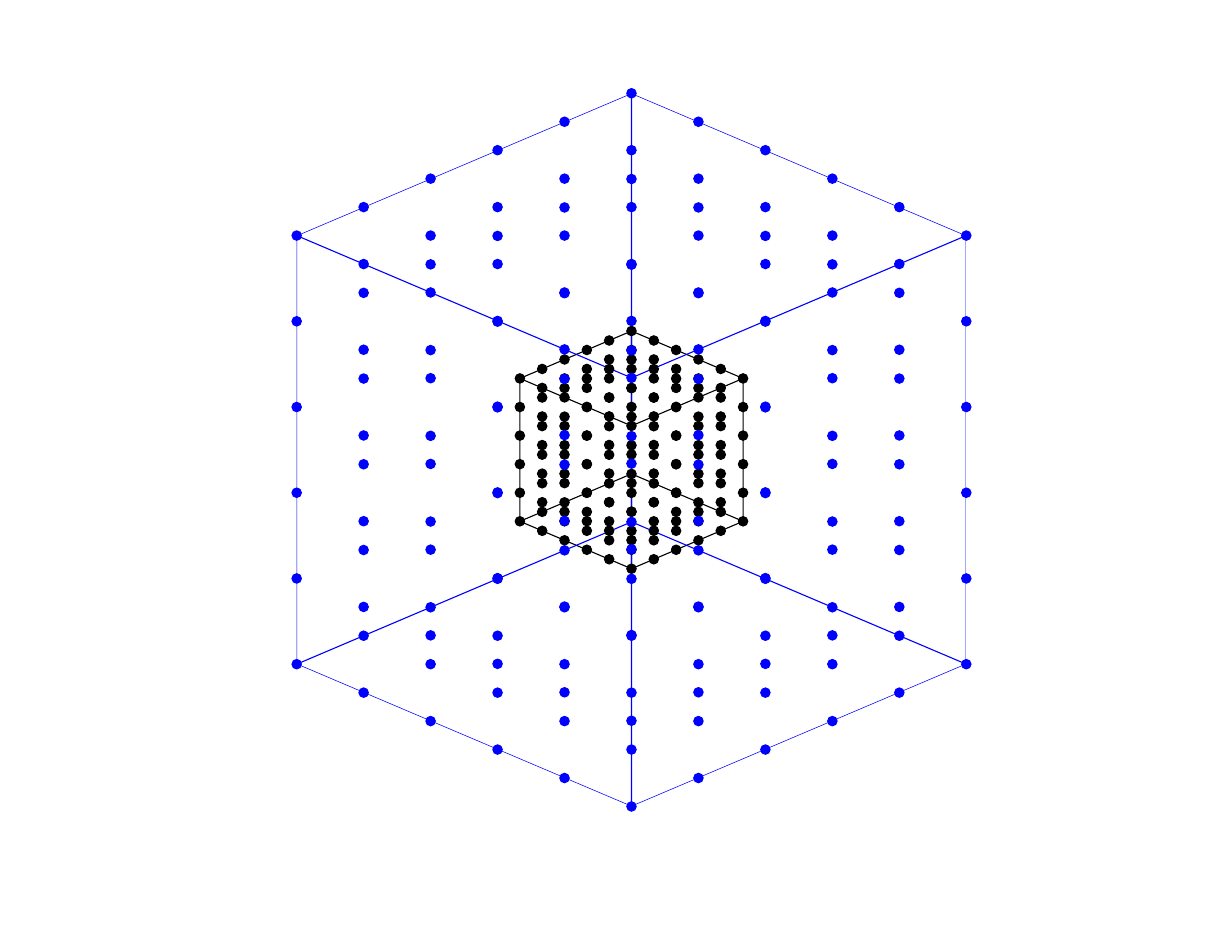
\begin{tikzpicture}

\begin{axis}[%
width=3.348in,
height=3.566in,
at={(1.345in,0.481in)},
scale only axis,
plot box ratio=1 1 1,
unbounded coords=jump,
xmin=-0.793615595547456,
xmax=1.67889551819639,
tick align=outside,
ymin=-0.793615595547456,
ymax=1.67889551819639,
zmin=-0.793615595547456,
zmax=1.67889551819639,
view={45}{25.15},
axis line style={draw=none},
ticks=none,
axis x line*=bottom,
axis y line*=left,
axis z line*=left
]
\addplot3 [color=black, only marks, mark size=1.7pt, mark=*, mark options={solid, black}]
 table[row sep=crcr] {%
0.0305547757004935	0.0305547757004935	0.0305547757004935\\
0.0305547757004935	0.195388849950083	0.0305547757004935\\
0.0305547757004935	0.360222924199673	0.0305547757004935\\
0.0305547757004935	0.525056998449263	0.0305547757004935\\
0.0305547757004935	0.689891072698853	0.0305547757004935\\
0.0305547757004935	0.854725146948443	0.0305547757004935\\
0.195388849950083	0.0305547757004935	0.0305547757004935\\
0.195388849950083	0.195388849950083	0.0305547757004935\\
0.195388849950083	0.360222924199673	0.0305547757004935\\
0.195388849950083	0.525056998449263	0.0305547757004935\\
0.195388849950083	0.689891072698853	0.0305547757004935\\
0.195388849950083	0.854725146948443	0.0305547757004935\\
0.360222924199673	0.0305547757004935	0.0305547757004935\\
0.360222924199673	0.195388849950083	0.0305547757004935\\
0.360222924199673	0.360222924199673	0.0305547757004935\\
0.360222924199673	0.525056998449263	0.0305547757004935\\
0.360222924199673	0.689891072698853	0.0305547757004935\\
0.360222924199673	0.854725146948443	0.0305547757004935\\
0.525056998449263	0.0305547757004935	0.0305547757004935\\
0.525056998449263	0.195388849950083	0.0305547757004935\\
0.525056998449263	0.360222924199673	0.0305547757004935\\
0.525056998449263	0.525056998449263	0.0305547757004935\\
0.525056998449263	0.689891072698853	0.0305547757004935\\
0.525056998449263	0.854725146948443	0.0305547757004935\\
0.689891072698853	0.0305547757004935	0.0305547757004935\\
0.689891072698853	0.195388849950083	0.0305547757004935\\
0.689891072698853	0.360222924199673	0.0305547757004935\\
0.689891072698853	0.525056998449263	0.0305547757004935\\
0.689891072698853	0.689891072698853	0.0305547757004935\\
0.689891072698853	0.854725146948443	0.0305547757004935\\
0.854725146948443	0.0305547757004935	0.0305547757004935\\
0.854725146948443	0.195388849950083	0.0305547757004935\\
0.854725146948443	0.360222924199673	0.0305547757004935\\
0.854725146948443	0.525056998449263	0.0305547757004935\\
0.854725146948443	0.689891072698853	0.0305547757004935\\
0.854725146948443	0.854725146948443	0.0305547757004935\\
0.0305547757004935	0.0305547757004935	0.195388849950083\\
0.0305547757004935	0.195388849950083	0.195388849950083\\
0.0305547757004935	0.360222924199673	0.195388849950083\\
0.0305547757004935	0.525056998449263	0.195388849950083\\
0.0305547757004935	0.689891072698853	0.195388849950083\\
0.0305547757004935	0.854725146948443	0.195388849950083\\
0.195388849950083	0.0305547757004935	0.195388849950083\\
0.195388849950083	0.854725146948443	0.195388849950083\\
0.360222924199673	0.0305547757004935	0.195388849950083\\
0.360222924199673	0.854725146948443	0.195388849950083\\
0.525056998449263	0.0305547757004935	0.195388849950083\\
0.525056998449263	0.854725146948443	0.195388849950083\\
0.689891072698853	0.0305547757004935	0.195388849950083\\
0.689891072698853	0.854725146948443	0.195388849950083\\
0.854725146948443	0.0305547757004935	0.195388849950083\\
0.854725146948443	0.195388849950083	0.195388849950083\\
0.854725146948443	0.360222924199673	0.195388849950083\\
0.854725146948443	0.525056998449263	0.195388849950083\\
0.854725146948443	0.689891072698853	0.195388849950083\\
0.854725146948443	0.854725146948443	0.195388849950083\\
0.0305547757004935	0.0305547757004935	0.360222924199673\\
0.0305547757004935	0.195388849950083	0.360222924199673\\
0.0305547757004935	0.360222924199673	0.360222924199673\\
0.0305547757004935	0.525056998449263	0.360222924199673\\
0.0305547757004935	0.689891072698853	0.360222924199673\\
0.0305547757004935	0.854725146948443	0.360222924199673\\
0.195388849950083	0.0305547757004935	0.360222924199673\\
0.195388849950083	0.854725146948443	0.360222924199673\\
0.360222924199673	0.0305547757004935	0.360222924199673\\
0.360222924199673	0.854725146948443	0.360222924199673\\
0.525056998449263	0.0305547757004935	0.360222924199673\\
0.525056998449263	0.854725146948443	0.360222924199673\\
0.689891072698853	0.0305547757004935	0.360222924199673\\
0.689891072698853	0.854725146948443	0.360222924199673\\
0.854725146948443	0.0305547757004935	0.360222924199673\\
0.854725146948443	0.195388849950083	0.360222924199673\\
0.854725146948443	0.360222924199673	0.360222924199673\\
0.854725146948443	0.525056998449263	0.360222924199673\\
0.854725146948443	0.689891072698853	0.360222924199673\\
0.854725146948443	0.854725146948443	0.360222924199673\\
0.0305547757004935	0.0305547757004935	0.525056998449263\\
0.0305547757004935	0.195388849950083	0.525056998449263\\
0.0305547757004935	0.360222924199673	0.525056998449263\\
0.0305547757004935	0.525056998449263	0.525056998449263\\
0.0305547757004935	0.689891072698853	0.525056998449263\\
0.0305547757004935	0.854725146948443	0.525056998449263\\
0.195388849950083	0.0305547757004935	0.525056998449263\\
0.195388849950083	0.854725146948443	0.525056998449263\\
0.360222924199673	0.0305547757004935	0.525056998449263\\
0.360222924199673	0.854725146948443	0.525056998449263\\
0.525056998449263	0.0305547757004935	0.525056998449263\\
0.525056998449263	0.854725146948443	0.525056998449263\\
0.689891072698853	0.0305547757004935	0.525056998449263\\
0.689891072698853	0.854725146948443	0.525056998449263\\
0.854725146948443	0.0305547757004935	0.525056998449263\\
0.854725146948443	0.195388849950083	0.525056998449263\\
0.854725146948443	0.360222924199673	0.525056998449263\\
0.854725146948443	0.525056998449263	0.525056998449263\\
0.854725146948443	0.689891072698853	0.525056998449263\\
0.854725146948443	0.854725146948443	0.525056998449263\\
0.0305547757004935	0.0305547757004935	0.689891072698853\\
0.0305547757004935	0.195388849950083	0.689891072698853\\
0.0305547757004935	0.360222924199673	0.689891072698853\\
0.0305547757004935	0.525056998449263	0.689891072698853\\
0.0305547757004935	0.689891072698853	0.689891072698853\\
0.0305547757004935	0.854725146948443	0.689891072698853\\
0.195388849950083	0.0305547757004935	0.689891072698853\\
0.195388849950083	0.854725146948443	0.689891072698853\\
0.360222924199673	0.0305547757004935	0.689891072698853\\
0.360222924199673	0.854725146948443	0.689891072698853\\
0.525056998449263	0.0305547757004935	0.689891072698853\\
0.525056998449263	0.854725146948443	0.689891072698853\\
0.689891072698853	0.0305547757004935	0.689891072698853\\
0.689891072698853	0.854725146948443	0.689891072698853\\
0.854725146948443	0.0305547757004935	0.689891072698853\\
0.854725146948443	0.195388849950083	0.689891072698853\\
0.854725146948443	0.360222924199673	0.689891072698853\\
0.854725146948443	0.525056998449263	0.689891072698853\\
0.854725146948443	0.689891072698853	0.689891072698853\\
0.854725146948443	0.854725146948443	0.689891072698853\\
0.0305547757004935	0.0305547757004935	0.854725146948443\\
0.0305547757004935	0.195388849950083	0.854725146948443\\
0.0305547757004935	0.360222924199673	0.854725146948443\\
0.0305547757004935	0.525056998449263	0.854725146948443\\
0.0305547757004935	0.689891072698853	0.854725146948443\\
0.0305547757004935	0.854725146948443	0.854725146948443\\
0.195388849950083	0.0305547757004935	0.854725146948443\\
0.195388849950083	0.195388849950083	0.854725146948443\\
0.195388849950083	0.360222924199673	0.854725146948443\\
0.195388849950083	0.525056998449263	0.854725146948443\\
0.195388849950083	0.689891072698853	0.854725146948443\\
0.195388849950083	0.854725146948443	0.854725146948443\\
0.360222924199673	0.0305547757004935	0.854725146948443\\
0.360222924199673	0.195388849950083	0.854725146948443\\
0.360222924199673	0.360222924199673	0.854725146948443\\
0.360222924199673	0.525056998449263	0.854725146948443\\
0.360222924199673	0.689891072698853	0.854725146948443\\
0.360222924199673	0.854725146948443	0.854725146948443\\
0.525056998449263	0.0305547757004935	0.854725146948443\\
0.525056998449263	0.195388849950083	0.854725146948443\\
0.525056998449263	0.360222924199673	0.854725146948443\\
0.525056998449263	0.525056998449263	0.854725146948443\\
0.525056998449263	0.689891072698853	0.854725146948443\\
0.525056998449263	0.854725146948443	0.854725146948443\\
0.689891072698853	0.0305547757004935	0.854725146948443\\
0.689891072698853	0.195388849950083	0.854725146948443\\
0.689891072698853	0.360222924199673	0.854725146948443\\
0.689891072698853	0.525056998449263	0.854725146948443\\
0.689891072698853	0.689891072698853	0.854725146948443\\
0.689891072698853	0.854725146948443	0.854725146948443\\
0.854725146948443	0.0305547757004935	0.854725146948443\\
0.854725146948443	0.195388849950083	0.854725146948443\\
0.854725146948443	0.360222924199673	0.854725146948443\\
0.854725146948443	0.525056998449263	0.854725146948443\\
0.854725146948443	0.689891072698853	0.854725146948443\\
0.854725146948443	0.854725146948443	0.854725146948443\\
};
 \addplot3 [color=blue, only marks, mark size=1.7pt, mark=*, mark options={solid, blue}]
 table[row sep=crcr] {%
-0.793615595547456	-0.793615595547456	-0.793615595547456\\
-0.793615595547456	-0.299113372798686	-0.793615595547456\\
-0.793615595547456	0.195388849950083	-0.793615595547456\\
-0.793615595547456	0.689891072698853	-0.793615595547456\\
-0.793615595547456	1.18439329544762	-0.793615595547456\\
-0.793615595547456	1.67889551819639	-0.793615595547456\\
-0.299113372798686	-0.793615595547456	-0.793615595547456\\
-0.299113372798686	-0.299113372798686	-0.793615595547456\\
-0.299113372798686	0.195388849950083	-0.793615595547456\\
-0.299113372798686	0.689891072698853	-0.793615595547456\\
-0.299113372798686	1.18439329544762	-0.793615595547456\\
-0.299113372798686	1.67889551819639	-0.793615595547456\\
0.195388849950083	-0.793615595547456	-0.793615595547456\\
0.195388849950083	-0.299113372798686	-0.793615595547456\\
0.195388849950083	0.195388849950083	-0.793615595547456\\
0.195388849950083	0.689891072698853	-0.793615595547456\\
0.195388849950083	1.18439329544762	-0.793615595547456\\
0.195388849950083	1.67889551819639	-0.793615595547456\\
0.689891072698853	-0.793615595547456	-0.793615595547456\\
0.689891072698853	-0.299113372798686	-0.793615595547456\\
0.689891072698853	0.195388849950083	-0.793615595547456\\
0.689891072698853	0.689891072698853	-0.793615595547456\\
0.689891072698853	1.18439329544762	-0.793615595547456\\
0.689891072698853	1.67889551819639	-0.793615595547456\\
1.18439329544762	-0.793615595547456	-0.793615595547456\\
1.18439329544762	-0.299113372798686	-0.793615595547456\\
1.18439329544762	0.195388849950083	-0.793615595547456\\
1.18439329544762	0.689891072698853	-0.793615595547456\\
1.18439329544762	1.18439329544762	-0.793615595547456\\
1.18439329544762	1.67889551819639	-0.793615595547456\\
1.67889551819639	-0.793615595547456	-0.793615595547456\\
1.67889551819639	-0.299113372798686	-0.793615595547456\\
1.67889551819639	0.195388849950083	-0.793615595547456\\
1.67889551819639	0.689891072698853	-0.793615595547456\\
1.67889551819639	1.18439329544762	-0.793615595547456\\
1.67889551819639	1.67889551819639	-0.793615595547456\\
-0.793615595547456	-0.793615595547456	-0.299113372798686\\
-0.793615595547456	-0.299113372798686	-0.299113372798686\\
-0.793615595547456	0.195388849950083	-0.299113372798686\\
-0.793615595547456	0.689891072698853	-0.299113372798686\\
-0.793615595547456	1.18439329544762	-0.299113372798686\\
-0.793615595547456	1.67889551819639	-0.299113372798686\\
-0.299113372798686	-0.793615595547456	-0.299113372798686\\
-0.299113372798686	1.67889551819639	-0.299113372798686\\
0.195388849950083	-0.793615595547456	-0.299113372798686\\
0.195388849950083	1.67889551819639	-0.299113372798686\\
0.689891072698853	-0.793615595547456	-0.299113372798686\\
0.689891072698853	1.67889551819639	-0.299113372798686\\
1.18439329544762	-0.793615595547456	-0.299113372798686\\
1.18439329544762	1.67889551819639	-0.299113372798686\\
1.67889551819639	-0.793615595547456	-0.299113372798686\\
1.67889551819639	-0.299113372798686	-0.299113372798686\\
1.67889551819639	0.195388849950083	-0.299113372798686\\
1.67889551819639	0.689891072698853	-0.299113372798686\\
1.67889551819639	1.18439329544762	-0.299113372798686\\
1.67889551819639	1.67889551819639	-0.299113372798686\\
-0.793615595547456	-0.793615595547456	0.195388849950083\\
-0.793615595547456	-0.299113372798686	0.195388849950083\\
-0.793615595547456	0.195388849950083	0.195388849950083\\
-0.793615595547456	0.689891072698853	0.195388849950083\\
-0.793615595547456	1.18439329544762	0.195388849950083\\
-0.793615595547456	1.67889551819639	0.195388849950083\\
-0.299113372798686	-0.793615595547456	0.195388849950083\\
-0.299113372798686	1.67889551819639	0.195388849950083\\
0.195388849950083	-0.793615595547456	0.195388849950083\\
0.195388849950083	1.67889551819639	0.195388849950083\\
0.689891072698853	-0.793615595547456	0.195388849950083\\
0.689891072698853	1.67889551819639	0.195388849950083\\
1.18439329544762	-0.793615595547456	0.195388849950083\\
1.18439329544762	1.67889551819639	0.195388849950083\\
1.67889551819639	-0.793615595547456	0.195388849950083\\
1.67889551819639	-0.299113372798686	0.195388849950083\\
1.67889551819639	0.195388849950083	0.195388849950083\\
1.67889551819639	0.689891072698853	0.195388849950083\\
1.67889551819639	1.18439329544762	0.195388849950083\\
1.67889551819639	1.67889551819639	0.195388849950083\\
-0.793615595547456	-0.793615595547456	0.689891072698853\\
-0.793615595547456	-0.299113372798686	0.689891072698853\\
-0.793615595547456	0.195388849950083	0.689891072698853\\
-0.793615595547456	0.689891072698853	0.689891072698853\\
-0.793615595547456	1.18439329544762	0.689891072698853\\
-0.793615595547456	1.67889551819639	0.689891072698853\\
-0.299113372798686	-0.793615595547456	0.689891072698853\\
-0.299113372798686	1.67889551819639	0.689891072698853\\
0.195388849950083	-0.793615595547456	0.689891072698853\\
0.195388849950083	1.67889551819639	0.689891072698853\\
0.689891072698853	-0.793615595547456	0.689891072698853\\
0.689891072698853	1.67889551819639	0.689891072698853\\
1.18439329544762	-0.793615595547456	0.689891072698853\\
1.18439329544762	1.67889551819639	0.689891072698853\\
1.67889551819639	-0.793615595547456	0.689891072698853\\
1.67889551819639	-0.299113372798686	0.689891072698853\\
1.67889551819639	0.195388849950083	0.689891072698853\\
1.67889551819639	0.689891072698853	0.689891072698853\\
1.67889551819639	1.18439329544762	0.689891072698853\\
1.67889551819639	1.67889551819639	0.689891072698853\\
-0.793615595547456	-0.793615595547456	1.18439329544762\\
-0.793615595547456	-0.299113372798686	1.18439329544762\\
-0.793615595547456	0.195388849950083	1.18439329544762\\
-0.793615595547456	0.689891072698853	1.18439329544762\\
-0.793615595547456	1.18439329544762	1.18439329544762\\
-0.793615595547456	1.67889551819639	1.18439329544762\\
-0.299113372798686	-0.793615595547456	1.18439329544762\\
-0.299113372798686	1.67889551819639	1.18439329544762\\
0.195388849950083	-0.793615595547456	1.18439329544762\\
0.195388849950083	1.67889551819639	1.18439329544762\\
0.689891072698853	-0.793615595547456	1.18439329544762\\
0.689891072698853	1.67889551819639	1.18439329544762\\
1.18439329544762	-0.793615595547456	1.18439329544762\\
1.18439329544762	1.67889551819639	1.18439329544762\\
1.67889551819639	-0.793615595547456	1.18439329544762\\
1.67889551819639	-0.299113372798686	1.18439329544762\\
1.67889551819639	0.195388849950083	1.18439329544762\\
1.67889551819639	0.689891072698853	1.18439329544762\\
1.67889551819639	1.18439329544762	1.18439329544762\\
1.67889551819639	1.67889551819639	1.18439329544762\\
-0.793615595547456	-0.793615595547456	1.67889551819639\\
-0.793615595547456	-0.299113372798686	1.67889551819639\\
-0.793615595547456	0.195388849950083	1.67889551819639\\
-0.793615595547456	0.689891072698853	1.67889551819639\\
-0.793615595547456	1.18439329544762	1.67889551819639\\
-0.793615595547456	1.67889551819639	1.67889551819639\\
-0.299113372798686	-0.793615595547456	1.67889551819639\\
-0.299113372798686	-0.299113372798686	1.67889551819639\\
-0.299113372798686	0.195388849950083	1.67889551819639\\
-0.299113372798686	0.689891072698853	1.67889551819639\\
-0.299113372798686	1.18439329544762	1.67889551819639\\
-0.299113372798686	1.67889551819639	1.67889551819639\\
0.195388849950083	-0.793615595547456	1.67889551819639\\
0.195388849950083	-0.299113372798686	1.67889551819639\\
0.195388849950083	0.195388849950083	1.67889551819639\\
0.195388849950083	0.689891072698853	1.67889551819639\\
0.195388849950083	1.18439329544762	1.67889551819639\\
0.195388849950083	1.67889551819639	1.67889551819639\\
0.689891072698853	-0.793615595547456	1.67889551819639\\
0.689891072698853	-0.299113372798686	1.67889551819639\\
0.689891072698853	0.195388849950083	1.67889551819639\\
0.689891072698853	0.689891072698853	1.67889551819639\\
0.689891072698853	1.18439329544762	1.67889551819639\\
0.689891072698853	1.67889551819639	1.67889551819639\\
1.18439329544762	-0.793615595547456	1.67889551819639\\
1.18439329544762	-0.299113372798686	1.67889551819639\\
1.18439329544762	0.195388849950083	1.67889551819639\\
1.18439329544762	0.689891072698853	1.67889551819639\\
1.18439329544762	1.18439329544762	1.67889551819639\\
1.18439329544762	1.67889551819639	1.67889551819639\\
1.67889551819639	-0.793615595547456	1.67889551819639\\
1.67889551819639	-0.299113372798686	1.67889551819639\\
1.67889551819639	0.195388849950083	1.67889551819639\\
1.67889551819639	0.689891072698853	1.67889551819639\\
1.67889551819639	1.18439329544762	1.67889551819639\\
1.67889551819639	1.67889551819639	1.67889551819639\\
};
 \addplot3 [color=black]
 table[row sep=crcr] {%
0.0305547757004935	0.0305547757004935	0.0305547757004935\\
0.854725146948443	0.0305547757004935	0.0305547757004935\\
0.854725146948443	0.854725146948443	0.0305547757004935\\
0.0305547757004935	0.854725146948443	0.0305547757004935\\
0.0305547757004935	0.0305547757004935	0.0305547757004935\\
0.0305547757004935	0.0305547757004935	0.854725146948443\\
0.854725146948443	0.0305547757004935	0.854725146948443\\
0.854725146948443	0.854725146948443	0.854725146948443\\
0.0305547757004935	0.854725146948443	0.854725146948443\\
0.0305547757004935	0.0305547757004935	0.854725146948443\\
0.0305547757004935	0.0305547757004935	0.0305547757004935\\
nan	nan	nan\\
0.854725146948443	0.0305547757004935	0.0305547757004935\\
0.854725146948443	0.0305547757004935	0.854725146948443\\
nan	nan	nan\\
0.854725146948443	0.854725146948443	0.0305547757004935\\
0.854725146948443	0.854725146948443	0.854725146948443\\
nan	nan	nan\\
0.0305547757004935	0.854725146948443	0.0305547757004935\\
0.0305547757004935	0.854725146948443	0.854725146948443\\
};
 \addplot3 [color=blue]
 table[row sep=crcr] {%
-0.793615595547456	-0.793615595547456	-0.793615595547456\\
1.67889551819639	-0.793615595547456	-0.793615595547456\\
1.67889551819639	1.67889551819639	-0.793615595547456\\
-0.793615595547456	1.67889551819639	-0.793615595547456\\
-0.793615595547456	-0.793615595547456	-0.793615595547456\\
-0.793615595547456	-0.793615595547456	1.67889551819639\\
1.67889551819639	-0.793615595547456	1.67889551819639\\
1.67889551819639	1.67889551819639	1.67889551819639\\
-0.793615595547456	1.67889551819639	1.67889551819639\\
-0.793615595547456	-0.793615595547456	1.67889551819639\\
-0.793615595547456	-0.793615595547456	-0.793615595547456\\
nan	nan	nan\\
1.67889551819639	-0.793615595547456	-0.793615595547456\\
1.67889551819639	-0.793615595547456	1.67889551819639\\
nan	nan	nan\\
1.67889551819639	1.67889551819639	-0.793615595547456\\
1.67889551819639	1.67889551819639	1.67889551819639\\
nan	nan	nan\\
-0.793615595547456	1.67889551819639	-0.793615595547456\\
-0.793615595547456	1.67889551819639	1.67889551819639\\
};
 \end{axis}

\begin{axis}[%
width=5.833in,
height=4.375in,
at={(0in,0in)},
scale only axis,
xmin=0,
xmax=1,
ymin=0,
ymax=1,
axis line style={draw=none},
ticks=none,
axis x line*=bottom,
axis y line*=left
]
\end{axis}
\end{tikzpicture}%}
    \caption[A diagram representing the upwards and downwards equivalent surface for an arbitrary node with bounds given in black.]{A diagram representing the upwards and downwards equivalent surface for an arbitrary node with bounds given in black. Both surfaces are discredited by a $6 \times 6 \times 6$ set of quadrature points. The upwards equivalent surface (black) lies on the boundary of the node while the downward equivalent surface (blue) is a cube with sides 3 times larger and centred on the node. }
    \label{fig:UpandDownsurf}
\end{figure}

In order to be able to use these equivalent potential densities in our method, we form a quadrature rule over an equally spaced uniform Cartesian grid with $N_q$ quadrature point. While the number of quadrature points in the upwards and downwards equivalent surfaces does not need to be the same, for convenience we will take this to be the case. We will indicate the quadrature points [for?] the upwards equivalent potential for a node $B$ with $\{\bm{q}^{BU}_m\}$ for $m=1,\dots,N_q$ and $\{\bm{q}^{BD}_m\}$ for $m=1,\dots,N_q$ indicating the positions of the quadrature points for the downwards equivalent potential. Now each of these quadrature points has a corresponding equivalent potential denoted by $\{\bm{f}^{BU}(\bm{q}^{BU}_m)\}$ and $\{\bm{f}^{BD}(\bm{q}^{BD}_m)\}$ for the upward and downward equivalent potentials respectively. Writing the left-hand side of \cref{eq:upsurfint,eq:downsurfint} using this quadrature rule we obtain that
\begin{equation}
\label{eq:L2Mfar}
    \forall \;\bm{x} \in \mathcal{F}(B): \quad \bm{u}(\bm{x})= \frac{1}{8 \pi \mu} \sum_{m=1}^{N_{q}} A_{m}^{BU} S^\epsilon\left(\bm{x}, \bm{q}_{m}^{B U}\right) \bm{f}^{B U}\left(\bm{q}_{m}^{B U}\right)
\end{equation}
and the contribution to the velocity $\bm{u}(\bm{x})$ for $\bm{x} \in B$ from source points in $\mathcal{F}(B)$ as
\begin{equation}
\label{eq:L2Mnear}
    \forall \;\bm{x} \in B: \quad \bm{u}(\bm{x})= \frac{1}{8 \pi \mu} \sum_{m=1}^{N_{q}} A_{m}^{BD} S^\epsilon\left(\bm{x}, \bm{q}_{m}^{B D}\right) \bm{f}^{B D}\left(\bm{q}_{m}^{B D}\right)
\end{equation}
Where $\{A_{m}^{BU}\}$ and $\{A_{m}^{BD}\}$ are the corresponding quadrature weights of the upwards and downwards equivalent points respectively. We will not explicitly calculate these weights and will take them to be part of their corresponding equivalent potential. The advantage of using \cref{eq:L2Mnear,eq:L2Mfar} is to avoid the direct computation of source points and target points and instead use the quadrature points as an approximation of the particles within the box.

We note that the downward equivalent surface lies in the $\mathcal{F}(B)$ and the downward equivalent surface lies in $B$ and hence we obtain the following systems of equations
\begin{equation}
\label{eq:upsum}
    \sum_{m=1}^{N_{q}} A_{m}^{BU} S^\epsilon\left(\bm{q}^{BD}_{k}, \bm{q}_{m}^{B U}\right) \bm{f}^{B U}\left(\bm{q}_{m}^{B U}\right)=\sum_{{\bm{y}}_{n} \in B} S^\epsilon\left(\bm{q}^{BD}_{k}, {\bm{y}}_{n}\right) {\bm{f}}_{n} A({\bm{y}}_n), \quad k=1,\dots,N_q
\end{equation}
and
\begin{equation}
\label{eq:downsum}
    \sum_{m=1}^{N_{q}} A_{m}^{BD} S^\epsilon\left(\bm{q}^{BU}_{k}, \bm{q}_{m}^{B D}\right) \bm{f}^{B D}\left(\bm{q}_{m}^{B D}\right)=\sum_{{\bm{y}}_{n} \in \mathcal{F}(B)} S^\epsilon\left(\bm{q}^{BU}_{k}, {\bm{y}}_{n}\right) {\bm{f}}_{n} A({\bm{y}}_n), \quad k=1,\dots,N_q
\end{equation}
We will use \cref{eq:upsum,eq:downsum} to construct the upwards and downwards potential of all nodes through the approximation of the left-hand side of the equation.

\subsection{Evaluation}
The Fast Multipole method is based on two passes, one up the tree in order to construct the upwards equivalent surfaces from source potentials and a further downward pass where we construct the downward equivalent potentials before finally evaluating the velocities at the target points.

\subsubsection{Upward Pass}
The upwards pass involves the postorder traversal (see \cref{appendix:Tree}) of the tree from the smallest node up to the root node and solving \cref{eq:upsum} for each node. For each leaf node, we can evaluate the right-hand side of \cref{eq:upsum} directly. Now for each non-leaf node $B$ in the tree, instead of summing over all source points in the decedents of $B$ we can approximate its upwards equivalent surface from its children. We denote the children of $B$ as $C_l^B$ where $l=1,...,8$. As we have traversed the tree in post-order we know $\{\bm{f}^{C_l U}(\bm{q}^{C_lU}_m)\}$ for $l=1,\dots,8$ and $m=1,\dots,N_q$. Since $\{\bm{q}^{C_lU}_m\}$ lies within $\{\bm{q}^{BU}_m\}$ we have that the right-hand side of \cref{eq:upsum} can be approximated as
\begin{equation}
\label{eq:M2M}
    \sum_{l=1}^{8} \sum_{m=1}^{N_{q}} A_{m}^{C_{l} U} S^\epsilon\left(\bm{q}_{k}^{B D}, \bm{q}_{m}^{C_{l} U}\right) \bm{f}^{C_{l} U}\left(\bm{q}_{m}^{C_{l} U}\right), \quad k=1,\dots,N_q
\end{equation}
We refer to this as a multipole to multipole translation (M2M). This method of approximating the parents equivalent potential from its children is significantly more efficient, as, provided that the number of quadrature points is smaller than the capacity of the node $s$, the number of kernel evaluations is significantly reduced compared to when the equivalent surface was computed directly using the right hand side of \cref{eq:upsum}. We note that in both summations we have computed the velocities at the downward equivalent surface, this ensures the existence of the $\{\bm{f}^{BU}(\bm{q}^{BU}_m)\}$. In order to obtain these values, we simply solve the linear system created by \cref{eq:upsum}. This gives us a set of equivalent potentials for each node in the tree which approximates the effect of all source points contained within that nodes region.

\subsubsection{Downwards Pass}
The downward pass follows a similar structure to that of the upwards pass, however we now traverse down the octree using a pre-order traversal (see \cref{appendix:Tree}). We do not need to consider the root node on level 0 so we start our traversal on level 1. We will now be considering equation \cref{eq:downsum} and approximating the right-hand side before solving the linear system to obtain the downward equivalent potentials for all considered nodes.

For each non-root node $B$ we need to consider the effect of source points in the far-field. In order to consider these effects, we define the Multipole to Local translation (M2L) and the Local to Local translation (L2L) translation. The M2L translation computes the contribution to the downward equivalent potential to[of?] $B$ for a node $A$ in $\mathcal{F}(B)$. As points, $\{\bm{q}^{BU}_m\}$ are in the $\mathcal{F}(A)$ we can consider the contribution to the right-hand side as approximately
\begin{equation}
\label{eq:M2L}
\sum_{m=1}^{N_{q}} A_{m}^{A U} S^\epsilon\left(\bm{q}_{k}^{B U}, \bm{q}_{m}^{A U}\right) \bm{f}^{A U}\left(\bm{q}_{m}^{A U}\right), \quad k=1,\dots,N_q
\end{equation}
We use \cref{eq:M2L} to compute the effect of all nodes in the interaction list $I_V^B$. The effect of other nodes in $\mathcal{F}(B)$ are computed through the M2L transition where we pass information of distant source points from parent to child[does not make sense]. As we are in pre-order traversal, we have already computed the downward equivalent potential of the parent of $B$. We will call the parent $P$ and it's downward equivalent potential $\{\bm{f}^{PD}(\bm{q}^{PD}_m)\}$. As $B$ is by definition inside of $P$ we know that $\{\bm{q}^{BU}_m\}$ is in $\mathcal{N}(B)$ so we can use \cref{eq:L2Mnear} to calculate the contribution to the right-hand side of \cref{eq:downsum} as
\begin{equation}
\label{eq:L2L}
\sum_{m=1}^{N_{q}} A_{m}^{P D} S^\epsilon\left(\bm{q}_{k}^{B U}, \bm{q}_{m}^{P D}\right) \bm{f}^{P D}\left(\bm{q}_{m}^{P D}\right), \quad k=1,\dots,N_q
\end{equation}
These two summations approximate the contributions of source points in $\mathcal{F}(B)$ however, we need to consider the near field contributions on $\{\bm{f}^{B D}(\bm{q}^{BD}_m)\}$. For any non leaf node we have that $I_U^B = I_W^B = \emptyset$ where $\emptyset$ is the empty set. This means we only need to consider $I_X^B$ in our calculation of the downward equivalent potential $\{\bm{f^{BD}}(\bm{q}^{BD}_m)\}$. We will consider the effect of nodes in $I_U^B$ and $I_W^B$ when we compute the velocity at the target points in the next step. We could use the M2L transition \cref{eq:M2L} to approximate the forces, however as any node $A \in I_X^B$ is by definition a leaf node and in $\mathcal{N}(B)$, we will consider the effects of its source points directly through the summation
\begin{equation}
\label{eq:X}
    \sum_{A_i \in I_X^B} \sum_{{\bm{x_0}}_n\in A_i} S^\epsilon\left(\bm{q}^{BU}_{k}, {\bm{x_0}}_{n}\right) {\bm{f_0}}_{n}, \quad k=1,\dots,N_q
\end{equation}

Having obtained approximations for the right-hand side of \cref{eq:downsum} we solve the linear system to find the values of $\{\bm{f}^{BD}(\bm{q}^{BD}_m)\}$ at the quadrature points.

Now we consider the leaf nodes of the system where we solve to find the velocity of the fluid at the target points. We can consider the leaf nodes in any order as the calculations for each leaf node are independent of each other even though they may lie on different levels of the Octree. In order to compute the velocity at the target points, we need to consider all points in $\mathcal{N}(B)$ and $\mathcal{F}(B)$. In the computation of  $\{\bm{f}^{BD}(\bm{q}^{BD}_m)\}$ we approximated the effect of points in $I_V^B$ and $I_X^B$ and source points outside of the interaction lists of node $B$. We can compute this effect though \cref{eq:L2Mnear}, we then need to consider the remaining source points in $I_U^B$ and $I_W^B$. We compute the effect of nodes in $I_W^B$ by writing the right-hand side of \cref{eq:L2Mfar} as
\begin{equation*}
    \frac{1}{8 \pi \mu} \sum_{m=1}^{N_{q}} A_{m}^{AU} S^\epsilon\left(\bm{x}, \bm{q}_{m}^{A U}\right) \bm{f}^{A U}\left(\bm{q}_{m}^{A U}\right)
\end{equation*}
for each node $A$ in $I_W^B$. We do this as for any node $A \in I_W^B$ as we know that $B \in I_X^A \in \mathcal{F}(A)$. We compute the effects of sources in $I_U^B$ which we do through
\begin{equation}
\label{eq:U}
    \bm{u}(\bm{x}) = \sum_{{\bm{y}}_n\in A} S^\epsilon(\bm{x},{\bm{y}}_n){\bm{f}}_n
\end{equation}
where $A \in I_U^B$.

After summing these contributions together we have constructed an approximation for the velocities at all target points considering the effects of all source points.

\subsection{Parallelisation}
The nature of Octree traversal lends itself to easy parallelisation, in both [directions of?] tree traversal we need either to have computed the upwards equivalent surface for the upwards pass or the computation of the parents downward equivalent surface. This means we do not need to follow post and pre-order traversal exactly as long as the required nodes are already computed. Due to the way in which the Octree is structured we know that all children are in the level below their parent so in both traversal [directions?] we can compute all nodes on the same level in parallel. In our implementation we use MATLAB's built in [a?] parfor operator from the Parallel Computing Toolbox to parallelise the loop over nodes on the same level. Table \ref{tab:CPUparalisation} shows the computation time in seconds for the computation of velocities given forces randomly distributed between 0 and 1. At all degrees of freedom we see an increase in the computation [time?], particularly at larger particles numbers, where parallelisation with 20 CPU cores allows for the KIFMM to compute the matrix vector product four times faster than when single threaded. While this is still far from perfect parallelisation, where we would expect to see the computation achieve a scaling efficiency of 5\% it still allows for much larger problems to be tackled as seen in \cref{fig:DirectProduct}. One particular downside of using MATLABs built in parfor is the increase in computation time achieved when 2 cores are used. This is due to MATLAB's implantation of the parfor operator, creating copies of the data it is using, this creates unnecessary copies of certain variables which increases the memory overhead when creating and using multiple threads. In order to remove these languages[obstacles?] we would need to move to a programming language which allows for pointers and the sharing of memory across multiple threads.

\begin{table}[ht]
    \centering
    \setlength{\tabcolsep}{6pt}
    \renewcommand{\arraystretch}{1.4}
    \small
    \begin{tabular}{c|lllllllllll}
     & \multicolumn{8}{l}{Scalar degrees of freedom} \\ \cline{2-9}
    \# of Cores & 488 & 5048 & 14408 & 28568 & 47528 & 213860 & 71288 & 99848 \\ \hline
    1 & 2.3889 & 14.141 & 10.725 & 31.671 & 76.755 & 107.15 & 159.54 & 274.34 \\
    2 & 1.1993 & 14.576 & 20.099 & 58.968 & 142.76 & 187.6 & 284.14 & 461.42 \\
    4 & 0.74177 & 7.892 & 10.643 & 31.724 & 74.996 & 98.82| & 151.07 & 242.26 \\
    6 & 0.78375 & 5.5193 & 7.5 & 22.281 & 51.961 & 68.328 & 104.45 & 168.65 \\
    8 & 0.66376 & 4.453 & 6.1626 & 17.997 & 40.65 & 55.064 & 81.835 & 132.26 \\
    10 & 0.6275 & 3.9803 & 5.1824 & 14.717 & 33.258 & 45.832 & 66.832 & 108.51 \\
    12 & 0.7658 & 3.7198 & 4.5536 & 13.593 & 28.836 & 38.159 & 58.441 & 94.983 \\
    14 & 0.60301 & 3.2507 & 4.1167 & 13.605 & 24.861 & 33.947 & 52.119 & 86.991 \\
    16 & 0.70194 & 3.0117 & 3.7601 & 12.081 & 23.636 & 31.33 & 47.6 & 75.986 \\
    18 & 0.69311 & 2.6899 & 3.4468 & 11.447 & 20.864 & 28.822 & 44.773 & 71.033 \\
    20 & 0.39093 & 2.9771 & 3.5109 & 12.049 & 19.872 & 27.087 & 41.699 & 65.026
    \end{tabular}
    \caption{CPU KIFMM computation time in sections for the Nyström method on a sphere with varying degrees of freedom}
    \label{tab:CPUparalisation}
\end{table}

\subsubsection{Use of GPU's in KIFMM}
Another attempt at improving the computation time of the KIFMM method is the use of GPU accelerated matrix multiplication. The design and architecture of GPU's allows for the computation of highly parallelisable tasks such as matrix multiplication to be computed significantly quicker. Passive GPU acceleration, where the use of MATLAB's built in gpuArray function allows for the acceleration of large numbers of MATLAB's built in functions such as the computation of matrix vector products and the use of the mldivide ($\backslash$) operator to solve linear systems. Within the method of regularised [what?] it has seen some success, with the time taken for the computation of large systems being reduced by nearly 7 times \cite{Gallagher2020}. The limiting factor of GPU computation is the limied memory available to the GPU, which is typically about 8-16GB compared to the hundreds of GB which are available to high end workstations and clusters. While block computation of matrix vector products allows for very large systems to be computed, the solving of linear systems though methods like LU decomposition need the whole matrix to be stored on the GPU. This memory limitation along with MATLAB's need to create a copy of variables per thread, proves hard to easily implement efficiently and in our implementation we opt to only accelerate the matrix vector products and LU decompositions needed for the M2L (\cref{eq:M2L}), M2M (\cref{eq:M2M}) and L2L (\cref{eq:L2L}) by passing only the required data for each transition and gathering it back to the CPU for further processing. This keeps the memory requirement on the GPU low, however it is not optimal, as data transfer to and from the GPU is slow. The results from this attempt can be seen in \cref{tab:GPUparalisation} where we see computational speeds increased from both parallelisation and GPU computation. We see about a 20\% increase in performance from using a single core. A more single-thread optimised version could see this computation time improved as we would not need to deal with multiple copies of arrays. This was not implemented as our focus was more on CPU parallelisation on HPC clusters. At medium sized systems of about 80000 particles we do see that our GPU implementation has similar computation times to that of our 20 core CPU results on much more modest hardware. More focused GPU optimisation has been widely explored for standard FMM with a version which almost entirely runs on the GPU now being available \cite{Yokota,Hamada200942Turbulence,Wilson2021ATraversal,Kohnke2020AAccuracy}, however little work has been done on the kernel independent method and could be be explored in future work.

\begin{table}[ht]
    \centering
    \setlength{\tabcolsep}{6pt}
    \renewcommand{\arraystretch}{1.4}
    \small
    \begin{tabular}{c|lllllllllll}
     & \multicolumn{8}{l}{Scalar degrees of freedom} \\ \cline{2-9}
    \# of Cores & 488 & 5048 & 14408 & 28568 & 47528 & 213860 & 71288 & 99848 \\ \hline
    1 & 0.98392 & 7.0386 & 8.3094 & 28.004 & 54.947 & 82.189 & 123.91 & 228.8 \\
    2 & 2.3513 & 4.0862 & 4.9127 & 15.912 & 31.957 & 47.295 & 70.942 & 133.95 \\
    4 & 2.2249 & 2.6397 & 3.2986 & 10.581 & 21.694 & 32.474 & 49.041 & 92.296 \\
    6 & 2.1567 & 2.3276 & 3.0579 & 9.1999 & 18.986 & 28.488 & 43.26 & 82.989 \\
    8 & 1.9829 & 2.1696 & 2.826 & 8.667 & 17.997 & 27.007 & 40.617 & 78.12 \\
    10 & 1.9643 & 2.0454 & 2.7493 & 8.2972 & 17.257 & 26.27 & 39.814 & 76.049 \\
    12 & 1.9107 & 3.5556 & 2.6386 & 8.2162 & 16.864 & 25.82 & 39.411 & 75.117 \\
    \end{tabular}
    \caption{GPU KIFMM computation time in sections for the Nyström method on a sphere with varying degrees of freedom}
    \label{tab:GPUparalisation}
\end{table}



\subsection{Comparison of KIFMM with the Direct Product}
In order to assess the performance benefit of the KIFMM for the evaluation of N-body problems using the regularised stokeslet kernel, we will perform simple calculations on both machine (M1) and (M2) (\cref{appendix:Hardware}). To compare the computation times we will be calculating the grand resistance matrix of a sphere at various scalar degrees of freedom using both KIFMM and the direct product, and GMRES to compute the inverse, to allow for more accurate comparison of the results. GMRES (\cref{appendix:GMRES}) was set to converge to a relative tolerance of $1e-6$ and the KIFMM having a maximum of 500 particles per node with 152 quadrature points per node. This provides a fast method while limiting the error associated with the equivalent surfaces. In order to check that both methods are similar we will also compute the relative error compared to the exact solution using \cref{eq:RelativeError}. [Needs a better explanation]

\begin{figure}[ht]
     \centering
     \begin{subfigure}[b]{0.49\textwidth}
         \centering
         \includegraphics[width=\textwidth]{Images/KIFMM/Graphs/DirectProductCompTime.pdf}
         \caption{Computation time for computing the Grand Resistance matrix for a sphere at varying Scalar degrees of Freedom}
         \label{fig:DirectProductCompTime}
     \end{subfigure}
     \hfill
     \begin{subfigure}[b]{0.49\textwidth}
         \centering
         \includegraphics[width=\textwidth]{Images/KIFMM/Graphs/DirectProductComperror.pdf}
         \caption{Relative error in computation of Grand Resistance error at various scalar degrees of freedom}
         \label{fig:DirectProductComperror}
     \end{subfigure}
        \caption{Computation time and error for calculating the grand resistance matrix of a sphere using the KIFMM and Direct product methods.}
        \label{fig:DirectProduct}
\end{figure}

Figure \ref{fig:DirectProductComperror} shows that all methods performed similarly when comparing their relative error from the exact solution. The increase in the error beyond $73000$ scalar degrees of freedom can be attributed to the $\mathcal{O}(P\epsilon^{-1/P} h^{1-P})$ error for any integer $P>3$. More important is the error between the two solutions which maintained an absolute difference of less than $1e-5$ at all scalar degrees of freedom considered. Computation times differ more, with the CPU implementation of the direct product taking significantly longer than all other implementations. As expected, the direct product methods follow an order $N^2$ relation, with the GPU implementation growing much more slowly. The KIFMM methods grow  order $N$, with the CPU method out performing our current GPU implementation. We would predict that this will continue to grown linearly for a given tolerance, as the number of GMRES iterations required to converge will grow slower than the number of scalar degrees of freedom. Understanding that the KIFMM method can perform the matrix vector operations needed to solve the system quicker than the direct product, we will explore how changes to the KIFMM internal parameters affect this method's accuracy. 

\begin{figure}[ht]
     \centering
     \begin{subfigure}[b]{0.49\textwidth}
         \centering
         \includegraphics[width=\textwidth]{Images/KIFMM/Graphs/QuadPointsTime.pdf}
         \caption{Computation time for computing the Grand Resistance matrix for a sphere at varying Scalar degrees of Freedom}
         \label{fig:QuadPointsTime}
     \end{subfigure}
     \hfill
     \begin{subfigure}[b]{0.49\textwidth}
         \centering
         \includegraphics[width=\textwidth]{Images/KIFMM/Graphs/QuadPointsError.pdf}
         \caption{Relative error in computation of Grand Resistance error at various scalar degrees of freedom}
         \label{fig:QuadPointsError}
     \end{subfigure}
        \caption{Computation time and error for calculating the grand resistance matrix of a sphere using the KIFMM using $4\times4\times4$,$6\times6\times6$,$8\times8\times8$ Cartesian grids.}
        \label{fig:QuadPoints}
\end{figure}

As shown in \cref{fig:QuadPointsTime} the kernel independent fast multi pole method [KIFMM] becomes more costly when a finer mesh with more quadrature points is used as the size of the linear systems which need to be solved increases. While the computation time of the problem increases, the error associated with the method decreases as the two integrals \cref{eq:upsurfint,eq:downsurfint} become more accurately approximated. For most simulations in this paper a $6\times6\times6$ Cartesian grid was used for the equivalent surfaces as it provides accurate results with a reasonable computation time at all degrees of freedom we will consider. Note that if we had considered a finer quadrature based on a larger Cartesian grid the KIFMM method is still more efficient than the direct product for most scalar degrees of freedom, particularly when using CPU computation. 

The results for a particular choice in node capacity show a more varied and less defined choice which varies more with the particular problem being tackled [not clear what you are trying to say!]. The data in \cref{fig:NodeCap} was generated based on a fixed $6\times6\times6$ cartesian grid for the equivalent surface and the maximum node capacity changed when generating the Octree. All experiments show similar results for the error achieved, with smaller node capacities having fractionally better results as the initial equivalent surfaces form a better representation of the contained force points. In most cases we see a trend where larger node capacities have shorter computation times, however this does not always hold for smaller systems where the generation of the equivalent surfaces at the root nodes dominates due to the larger systems [does not make sense!]. 

\begin{figure}[ht]
     \centering
     \begin{subfigure}[b]{0.49\textwidth}
         \centering
         \includegraphics[width=\textwidth]{Images/KIFMM/Graphs/NodeCapTime.pdf}
         \caption{Computation time for computing the Grand Resistance matrix for a sphere at varying Scalar degrees of Freedom}
         \label{fig:NodeCapTime}
     \end{subfigure}
     \hfill
     \begin{subfigure}[b]{0.49\textwidth}
         \centering
         \includegraphics[width=\textwidth]{Images/KIFMM/Graphs/NodeCapError.pdf}
         \caption{Relative error in computation of Grand Resistance error at various scalar degrees of freedom}
         \label{fig:NodeCapError}
     \end{subfigure} \\
     \begin{subfigure}[b]{0.49\textwidth}
         \centering
         \includegraphics[width=\textwidth]{Images/KIFMM/Graphs/NodeCapError2.pdf}
         \caption{Relative error in computation of Grand Resistance error at various scalar degrees of freedom}
         \label{fig:NodeCapTime2}
     \end{subfigure}
        \caption{Computation time and error for calculating the grand resistance matrix of a sphere using the KIFMM and Direct product methods.}
        \label{fig:NodeCap}
\end{figure}
